\section{Funktioner}

\subsection{Definitioner}

\paragraph{Definition av en funktion}

Låt $X, Y$ vara mängder. En funktion $f: X\to Y$ är ett sätt att till varje element $x \in X$ tilldela ett välbestämt element $y\in Y$. Vi säger att $x$ avbildas på $y$ och att $y$ är bilden av $x$. $x$ kallas argumentet till $f$. $X$ kallas funktionens definitionsmängd, och betecknas även $D_f$. $Y$ kallas funktionen målmängd.

\paragraph{Värdemängd}

Värdemängden till $f: X\rightarrow Y$ definieras som:
\begin{align}
	V_f=\left \{y\in Y: y=f(x)\textnormal{ för något }x\in X\right \}\nonumber
\end{align}
alltså alla värden $f$ antar.

\paragraph{Injektivitet}

$f$ är injektiv om det för varje $x_1, x_2 \in X$ gäller att om $f(x_1)=f(x_2)$ så är $x_1=x_2$.

\paragraph{Surjektivitet}

$f$ är surjektiv om $V_f=Y$.

\paragraph{Bijektivitet}

Om $f$ är injektiv och surjektiv, är $f$ bijektiv.

\paragraph{Inversa funktioner}

Låt $f: X \to Y$ vara en bijektiv funktion. Inversen till $f$ är avbildningen $f^{-1}: Y\to X$ som ges av $f^{-1}(y)=x$, där $y=f(x)$. Funktioner som har en invers kallas inverterbara.

\paragraph{Växande och avtagande funktioner}

En funktion $f$ är växande på en mängd $M\in D_f$ om det för varje $x,y\in M: x<y$ gäller att $f(x)\leq f(y)$. Om $M=D_f$ kallas $f$ växande. Avtagande funktioner definieras analogt.

\paragraph{Strängt växande och avtagande funktioner}

En funktion $f$ är strängt växande på en mängd $M\in D_f$ om det för varje $x,y\in M: x<y$ gäller att $f(x)<f(y)$. Om $M=D_f$ kallas $f$ strängt växande. Strängt avtagande funktioner definieras analogt.

\paragraph{Monotona funktioner}

Om en funktioner är antingen strängt växande respektiva strängt avtagande eller växande respektiva avtagande i ett intervall, är den strängt monoton respektiva monoton.

\paragraph{Uppåt och nedåt begränsade funktioner}
En funktion $f$ är uppåt begränsad om $V_f$ är uppåt begränsad. Nedåt begränsade funktioner definieras analogt. Om funktioner saknar övre eller nedra begrensning är den uppåt eller nedåt obegränsad.

\paragraph{Minima och maxima}
En funktion $f$ har ett lokalt maximum i $x_0$ om det finns en omgivning $I$ till $x_0$ så att $f(x)\leq f(x_0)$ för alla $x\in I\cap D_f$. Det analoga gäller för ett lokalt minimum. Om $f$ har antingen ett lokalt maximum eller minimum i $x_0$ har $f$ ett lokalt extrempunkt i $f$.

\paragraph{Globala maxima och minima}
En funktion $f$ har ett globalt maximum i $x_0$ om $f(x)\leq f(x_0$ för varje $x\in D_f$.

\paragraph{Trigonometriska funktioner}

Betrakta enhetssirkeln i figur \ref{fig:unit_circle}, med radie $1$.

\begin{figure}[!ht]
	\centering
	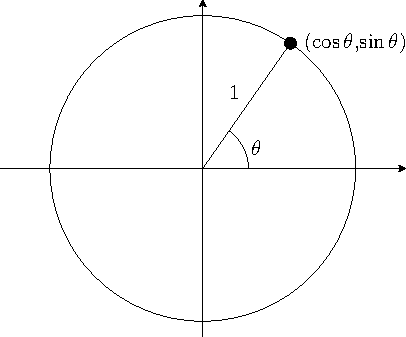
\includegraphics[width=0.5\linewidth]{./Images/unit_circle/unit_circle.pdf}
	\caption{Enhetscirkeln.}
	\label{fig:unit_circle}
\end{figure}

Man tenker sig en punkt på cirkeln enligt figuren, var linjen från cirkelns centrum till cirkeln bildar en vinkel $\theta$ med $x$-axeln. Denna vinkeln startar när punkten på cirkeln ligger på den positiva sidan av $x$-axeln, och ökar moturs. Från denna konstruktionen definieras $\sin$ och $\cos$ utifrån $x$- och $y$-koordinaterna till punkten för en given $\theta$, var $\theta$ mäts i radianer. Vi definierar även $\tan\theta=\frac{\sin\theta}{\cos\theta}$.

Från definitonerna ser vi at $\sin x$ och $\cos x$ är definierade för alla $x\in\R$, medan $\tan x$ är definierad för alla $x\neq \frac{\pi}{2}n, n\in\Z$.

\paragraph{Radianer}

Radianer är ett mått på vinklar som är baserad på enhetscirkeln. Om man tenker sig att punkten i figur \ref{fig:unit_circle} beväger sig från startpunktet och till nån 

\paragraph{Trigonometriska funktioners egenskaper}

Från definitionen av dom trigonometriska funktionerna följer många egenskaper vid dissa. Några essensiella är listad under:

\begin{align*}
	&\cos^2x + \sin^2x = 1\\
	&\sin\left(\theta + 2\pi n\right) = \sin\theta\\
	&\cos\left(\theta + 2\pi n\right) = \cos\theta\\
	&\sin\left(\theta - \frac{\pi}{2}\right) = \cos\theta\\
	&\cos\left(\theta + \frac{\pi}{2}\right) = \sin\theta\\
	&\sin\left(-\theta\right) = -\sin\theta\\
	&\cos\left(-\theta\right) = -\cos\theta\\
	&\sin\left(\theta+\pi\right) = -\sin\theta\\
	&\cos\left(\theta+\pi\right) = -\cos\theta
\end{align*}

\paragraph{Inversa trigonometriska funktioner}

Låt $f:\left[-\frac{\pi}{2},\frac{\pi}{2}\right]\to [-1,1]$ sådan att $f(x)=\sin x$. Inversen till denna funktionen betecknas $f^{-1}(x)=\arcsin x$.

Låt $f:[0,\pi]\to [-1,1]$ sådan att $f(x)=\cos x$. Inversen till denna funktionen betecknas $f^{-1}(x)=\arccos x$.

Låt $f:(-\infty,\infty)\to \left(-\frac{\pi}{2},\frac{\pi}{2}\right)$ sådan att $f(x)=\tan x$. Inversen till denna funktionen betecknas $f^{-1}(x)=\arctan x$.

\paragraph{Exponentialfunktionen}

I häftet definieras inte exponentialfunktionen $a^x, a>1$, utan den antas vara en strängt växande funktion med värdemängd $(0,\infty)$ som uppfyller
\begin{align*}
	&a^0 = 1\\
	&a^1 = a\\
	&a^{x + y} = a^x a^y\\
	&a^{-x} = \frac{1}{a^x}\\
	&\left(a^x\right)^y = a^{xy}
\end{align*}

\paragraph{Logaritmfunktionen}

Låt $f:\mathbb{R}\to (0,\infty)$ sådan att $f(x) = a^x$ för något $a > 1$. Inversen till denna funktionen betecknas som $f^{-1}(x) = \log_a x$.

\paragraph{Absolutbelopp}

Absolutbeloppet definieras som $\abs{x} = \sqrt{x^2}$. Detta impliserar att
\begin{align*}
	\abs{x} =
	\begin{cases}
		-x, & x < 1\\
		x,  & x \geq 1
	\end{cases}
\end{align*}
 
\paragraph{Kontinuitet}
Låt $f$ vara en reellvärd funktion med $D_f\subset\R$, sådan att varje punkterad omgivning till $x = a$ innehåller punkter från $D_f$ och $a\in D_f$. $f$ är kontinuerlig i $a$ om
\begin{align*}
	\lim\limits_{x\to a}f(x) = f(a).
\end{align*}

\paragraph{Likformig kontinuitet}
$f$ är likformig kontinuerlig på intervallet $I$ om det för varje $\varepsilon > 0$ existerar ett $\delta > 0$ sådant att $\abs{f(x) - f(y)} < \varepsilon$ för varje $x, y\in I$ som uppfyller att $\abs{x - y} < \delta$.

\paragraph{Konvexitet}
En funktion $f$ är konvex i $[a, b]$ om det för varje $x_1, x_2\in [a, b]$ gäller att
\begin{align*}
	f(tx_1 + (1 - t)x_2)\leq tf(x_1) + (1-t)f(x_2), t\in [0, 1].
\end{align*}

\paragraph{Konkavitet}
En funktion $f$ är konkav  i $[a, b]$ om $-f$ är konvex i $[a, b]$.

\paragraph{Inflexionspunkt}
Låt $f$ vara en funktion definierad på ett intervall $I$. En punkt $x_0\in I$ sägs vara en inflexionspunkt till $f$ om det finns ett $\delta > 0$ sådan att $f$ är konvex i $[x_0 - \delta, x_0]$ eller $[x_0, x_0 + \delta]$ och konkav i det andra.

\paragraph{Lodräta asymptoter}
Linjen $x = a$ är en lodrät asymptot till $f$ om $f(x)$ går mot $\infty$ eller $-\infty$ när $x\to a^{-}$ eller $x\to a^{+}$.

\paragraph{Sneda asymptoter}
Linjen $y = kx + m$ är en sned asymptot till $f$ om
\begin{align*}
	\limit{x}{\infty}(f(x) - (kx + m)) = 0
\end{align*}
eller
\begin{align*}
	\limit{x}{-\infty}(f(x) - (kx + m)) = 0.
\end{align*}
Givet att $f$ har en sned asymptot, ger definitionen
\begin{align*}
	k = \limit{x}{\infty}\frac{f(x)}{k}, m = \limit{x}{\infty}(f(x) - kx)
\end{align*}
eller analogt om asymptoten är vid $-\infty$.

\paragraph{Stora ordo vid oändligheten}
Låt $f, g$ vara funktioner definierade i $(a, \infty)$ för något $a$. $f$ tillhör stora ordo av $g$ då $x\to\infty$, med notation $f(x) = \Ordo{g(x)}$, om det finns $M$ och $x_0$ så att
\begin{align*}
	\abs{f(x)}\leq M\abs{g(x)}
\end{align*}
för varje $x > x_0$.

\paragraph{Stora ordo kring en punkt}
Låt $f, g$ vara funktioner definierade i en omgivning till $a$. $f$ tillhör stora ordo av $g$ kring $a$, med notation $f(x) = \Ordo{g(x)}$, om det finns $M$ och $\delta > 0$ så att
\begin{align*}
	\abs{f(x)}\leq M\abs{g(x)}
\end{align*}
för varje $x\in(a - \delta, a + \delta)$.

\subsection{Satser}

\paragraph{Trigonometriska funktioner med vinkelsummor}
\begin{align*}
	\sin\left(x+y\right) = \sin x\cos y + \cos x\sin y\\
	\cos\left(x+y\right) = \cos x\cos y - \sin x\sin y
\end{align*}

\paragraph{Cosinussatsen}

Låt $a,b,c$ vara sidorna i en triangel och $\theta$ vinkeln där sidlängderna $a$ och $b$ möts. Då gäller att
\begin{align*}
	c^2=a^2+b^2-2ab\cos\theta
\end{align*}

\paragraph{Logaritmfunktionens egenskaper}

Låt $a > 1$. Då gäller att
\begin{align}
	&\log_a 1 = 0 \label{eq:log_1}\\
	&\log_a\left(xy\right) = \log_a\left(x\right) + \log_a\left(y\right) \label{eq:log_prod}\\
	&\log_a\left(x^y\right) = y\log_a\left(x\right) \label{eq:log_pow}
\end{align}

\proof
Alla identiteter är baserade på inverterbarheten till exponentialfunktionen - $a^{\log_a x} = x$ - och injektiviteten till exponentialfunktionen, samt reglerna som exponentialfunktionen uppfyllar.

Ekvation \ref{eq:log_1} fås från att $a^{\log_a 1} = 1$ och att $a^0 = 1$. Eftersom exponentialfunktionen är injektiv, är det bevisad.

Ekvation \ref{eq:log_prod} fås från att $a^{\log_a xy} = xy$ och att $a^{\log_a x + \log_a y} = a^{\log_a x}a^{\log_a y}=xy$.

Ekvation \ref{eq:log_pow} fås från att $a^{\log_a x^y} = x^y$ och att $a^{y\log_a x} = \left(a^{\log_a x}\right)^y = x^y$.

\paragraph{Absolutbeloppens egenskaper}

\begin{align}
	&\abs{xy} = \abs{x}\abs{y} \label{eq:abs_prod} \\
	&\abs{x + y} \leq \abs{x} + \abs{y} \label{eq:abs_sum}
\end{align}

\proof

\paragraph{Kontinuitet av samansatta funktioner}
Låt $f$ vara kontinuerlig i $b$ och låt $g(x)\to b$ när $x\to a$. Då gäller att
\begin{align*}
	\lim\limits_{x\to a}f(g(x)) = f(\lim\limits_{x\to a}g(x))
\end{align*}
givet att vänsterledet är definierat.

\proof

\paragraph{Kontinuitet och begränsning}\label{par:continuity_limited}
Låt $f: [a,b]\to\R$ vara en kontinuerlig funktion. Då är $f$ begränsad.

\proof

\paragraph{Inversfunktioners kontinuerlighet}
Låt $f: A\to B$ vara en kontinuerlig, inverterbar och strängt växande funktion. Då gäller att inversen $f^{1}: B\to A$ är kontinuerlig och strängt växande.

\proof

\paragraph{Elementära funktioners kontinuerlighet}
Elementära funktioner är kontinuerliga.

\proof

\paragraph{Kontinuerlighet av summa och produkt}
Summan och produktet av kontinuerliga funktioner är kontinuerlig.

\proof

\paragraph{Intervallhalvering}
låt $[a_i, b_i]$ vara intervall så att $[a_{i + 1}, b_{i + 1}]$ vid att låta en vara mittpunktet på $[a_i, b_i]$ och den andra vara oändrat. Då finns det ett unikt $x$ så att $x\in [a_i, b_i]$ för alla $i\in\N$.

\proof

\paragraph{Satsen om mellanliggande värde}
Låt $f$ vara kontinuerlig i $[a, b]$. Då antar $f$ alla värden mellan $f(a)$ och $f(b)$.

\proof
I fallet $f(a) = f(b)$ är beviset trivialt.

Anta att $f(a) < m < f(b)$ för något $m$ (ett analogt bevis gäller i motsatta fallet). Definiera $a_0 = a$ och $b_0 = b$, bilda intervallet $[a_0, b_0]$ och beräkna funktionsvärdet i mittpunktet. Om detta är större än $m$, välj $b_1$ till att vara mittpunktet och $a_1 = a_0$, eller motsatt i motsatt fall. Fortsätta så med intervallhalvering. Då har vi $f(a_i)\leq m\leq f(b)$ för varje $i\in\N$.

Mängden av alla $a_i$ är växande och uppåt begränsad av $b_i$, och mängden av alla $b_i$ är avtagande och nedåt begränsad av $a_i$. Vi kan da låta $j\to\infty$, och får $f(x)\leq m\leq f(x)\implies f(x) = m$ för något $x\in [a, b]$. Detta gäller för alla $m$ som uppfyllar kravet, och beviset är klart.

\paragraph{Största och minsta värden}
Låt $f: [a,b]\to\R$ vara en kontinuerlig funktion. Då finns $x_1, x_2\in [a,b]$ så att $\sup{V_f} = f(x_1)$ och $\inf{V_f} = f(x_2)$.

\proof
Vi vet enligt \ref{par:continuity_limited} att funktionens värdemängd är begränsad. Definiera $M = \sup V_f$, som då existerar, och anta att $M\neq f(x)$ på $[a, b]$. Då är funktionen $g$ så att
\begin{align*}
	g(x) = \frac{1}{M - f(x)}
\end{align*}
definierad på $[a, b]$, kontinuerlig och därmed begränsad. Då finns $C = \sup V_g$, och
\begin{align*}
	\frac{1}{M - f(x)}\leq X\implies f(x)\leq M - \frac{1}{C}.
\end{align*}
Enligt antagandet är $M > f(x)$, och då är $C$ positiv. Då är $M - \frac{1}{C} < M$, och vi har hittat en mindre övre begränsning för $f$. Detta motsäjer antagandet, och då måste det finns ett $x\in [a, b]$ så att $f(x) = M$.

Ett analogt bevis gäller för att visa att $f$ antar ett minsta värde.

\paragraph{Likformig kontinuitet och kontinuitet}
Låt $f$ vara kontinuerlig på $[a, b]$. Då är $f$ likformigt kontinuerlig på $[a, b]$.

\proof

\paragraph{Stora ordos egenskaper}
Låt $f, g$ vara funktioner sådana att $\Ordo{f(x)}, \Ordo{g(x)}$ är definierade kring en punkt eller vid $\infty$. Då gäller:
\begin{align*}
	\Ordo{f(x)}\Ordo{g(x)}    &= \Ordo{f(x)g(x)}, \\
	\Ordo{f(x)} + \Ordo{g(x)} &= \Ordo{\abs{f(x)} + \abs{g(x)}}.
\end{align*}

\proof